%%%%%%%%%%%%%%%%%%%%%%%%%%%%%%%%%%%%%%%%%%%%%%%%%%%%%%%%%%%%%%%%%%%%%%
%
%   PROJECT REPORT FOR "note0" APPLICATION
%   Updated Version - Based on Actual Codebase Implementation
%
%%%%%%%%%%%%%%%%%%%%%%%%%%%%%%%%%%%%%%%%%%%%%%%%%%%%%%%%%%%%%%%%%%%%%%

\documentclass[12pt, a4paper]{report}

%======================================================================
%   1. REQUIRED PACKAGES
%======================================================================
\usepackage{svg}
% --- Font and Spacing Configuration ---
\usepackage{mathptmx} % Use Times New Roman font for the entire report
\usepackage[T1]{fontenc}
\usepackage{setspace} % For line spacing
\onehalfspacing % Set line spacing to 1.5 lines for paragraphs

% --- Page Layout ---
\usepackage[a4paper, margin=1in]{geometry} % Standard A4 paper with 1-inch margins

% --- Heading and Title Customization ---
\usepackage{titlesec} % To customize chapter and section titles

% Chapter Title: Times New Roman 18, Bold, Center
\titleformat{\chapter}[display]
  {\normalfont\fontsize{18}{22}\bfseries\centering}
  {\chaptertitlename\ \thechapter}
  {20pt}
  {\fontsize{18}{22}\selectfont}

% Heading 2 (Section): Times New Roman 16, Bold, Left Aligned
\titleformat{\section}
  {\normalfont\fontsize{16}{19}\bfseries}
  {\thesection}
  {1em}
  {}
% Add 3 lines of spacing before a section heading
\titlespacing*{\section}{0pt}{3\baselineskip}{1\baselineskip}

% Heading 3 (Subsection): Times New Roman 14, Bold, Left Aligned
\titleformat{\subsection}
  {\normalfont\fontsize{14}{17}\bfseries}
  {\thesubsection}
  {1em}
  {}

% --- Figures, Tables, and Graphics ---
\usepackage{graphicx} % To include images
\usepackage{caption} % To customize captions
% Ensure table titles are ABOVE the table
\captionsetup[table]{position=top, singlelinecheck=false, font=small}
% Ensure figure titles are UNDER the figure
\captionsetup[figure]{position=bottom, singlelinecheck=false, font=small}

% --- Other useful packages ---
\usepackage{amsmath} % For mathematical equations
\usepackage{lipsum} % For generating placeholder text to meet page count
\usepackage{hyperref} % For clickable links in the PDF (optional)


%======================================================================
%   2. DOCUMENT START
%======================================================================
\begin{document}

% Ensure all body text is justified
\justifying

%======================================================================
%   i & ii. TOP COVER / TITLE PAGE
%======================================================================
% \begin{titlepage}
%     \centering
%     \vspace*{1cm}
    
%     {\Huge \bfseries note0: A  Note-Sharing Platform}
    
%     \vspace{1.5cm}
    
%     {\Large Project Report}
    
%     \vspace{1.5cm}
    
%     {\large Submitted in partial fulfillment of the requirements for the course}
    
%     \vspace{0.5cm}
    
%     {\large \textit{Object Oriented Programming}}
    
%     \vspace{2cm}
    
%     {\Large \bfseries By}
    
%     \vspace{1cm}
    
%     {\large
%     \begin{tabular}{ll}
%         Adharsh k & (Roll No.09) \\
%         Abhijith R & (Roll No.01) \\
%         Aswin R & (Roll No.54) \\ 
%     \end{tabular}
%     }
    
%     \vspace{2cm}
    
%     {\Large \bfseries Under the guidance of}
    
%     \vspace{1cm}
    
%     {\large Vijesh Sir}
    
%     {\large Assistant Prof.}
    
%     \vfill
    
%     % 
%     % To add your logo, upload an image file (e.g., logo.png) to Overleaf
%     % and uncomment the line below.
%     % \includegraphics[width=0.4\textwidth]{logo.png}
    
%     \vspace{1cm}
    
%     {\Large \bfseries Department of Computer Science and Engineering}
    
%     {\Large Abdul Kalam University}
    
%    % {\Large City, State - Pincode}
    
%     \vspace{1cm}
    
%     {\large October 2025}
    
% \end{titlepage}


%======================================================================
%   iii. CERTIFICATION PAGE
%======================================================================
\begin{center}
\textbf{PBCST304 OBJECT ORIENTED PROGRAMMING}\\[0.3cm]
\textbf{Micro Project Report}\\[0.3cm]
\textbf{on}\\[0.3cm]
\textbf{NOTE0- A  Note-Sharing Platform}\\[0.8cm]
\textbf{Submitted by}\\[0.3cm]
\textbf{ABHIJITH R(NSS24CS002)}\\[0.5cm]
\textbf{ADHARSH K (NSS24CS010)}\\[.5cm]
\textbf{ASWIN R(NSS24CS055)}\\[.5cm]
\end{center}
\date{Analysis Date: APRIL 21, 2025}
\begin{figure}[h] % h = here, t = top, b = bottom, etc.
  \centering
  \includegraphics[width=0.6\textwidth]{images/NSS_LOGO.jpg} % Change to your image name
   
  
\end{figure}
\begin{center}
    \textbf{\LARGE NSS COLLEGE OF ENGINEERING}\\[0.3cm]
    \Large
    \textbf{Govt. Aided College Affiliated to APJ Abdul Kalam Technological University}\\[0.3cm]
    \textbf{Approved by AICTE}\\[1cm]

    \includegraphics[width=0.3\textwidth]{images/NSS_LOGO.jpg} % logo again
    
    \vspace{1cm} % Add some space after the logo
    
    \parbox{0.9\textwidth}{
        \centering
        \textbf{Certified that this is a Bonafide report of work done in \textit{NOTE0} by \textbf{ABHIJITH R, ADHARSH K, ASWIN R} of this institution as prescribed by APJ Abdul Kalam Technological University, for the 3\textsuperscript{rd} Semester course in B.Tech in Computer Science and Engineering branch during the academic year 2024--2028.}
    }
\end{center}

\vfill % Pushes the signature block to the bottom

% --- First row of signatures (Guide and HOD) ---
\noindent % Prevents indentation
\begin{minipage}[t]{0.5\textwidth} % Left column
    \centering
    \vspace{2cm} % Space for the signature
    \dotfill \\ % Dotted signature line
    \textbf{Vijesh K} \\
    \textit{Project Guide}
\end{minipage}%
\begin{minipage}[t]{0.5\textwidth} % Right column
    \centering
    \vspace{2cm} % Space for the signature
    \dotfill \\ % Dotted signature line
    \textbf{Dr. Anuraj Mohan} \\
    \textit{Head of the Department}
\end{minipage}

\vspace{2cm} % Space between the rows

% --- Second row for External Examiner ---
\begin{center}
    \begin{minipage}{0.5\textwidth} % A centered box for the final signature
        \centering
        \vspace{2cm} % Space for the signature
        \dotfill \\ % Dotted signature line
        \textit{External Examiner}
    \end{minipage}
\end{center}
%======================================================================
%   iv. ACKNOWLEDGEMENT
%======================================================================
\chapter*{Acknowledgement}
\addcontentsline{toc}{chapter}{Acknowledgement}

We would like to express our sincere gratitude to our project guide, \textbf{Vijesh Sir}, for their invaluable guidance, constant encouragement, and insightful feedback throughout the duration of this project. Their expertise was instrumental in helping us navigate the technical challenges and successfully complete our work.
We would like to extend our heartfelt thanks to Principal \textbf{Dr. Saju N} for providing us with the
opportunity to undertake this project.
We are also thankful to our Head of Department, \textbf{Anuraj Mohan}, and all the faculty members of the Department of Computer Science and Engineering for providing us with the necessary resources and a conducive environment for learning and research.

Finally, we would like to thank our family and friends for their unwavering support and encouragement.

\vspace{2cm}
\begin{flushright}
    Adharsh k \\
    Abhijith R \\
    Aswin R \\
\end{flushright}

\newpage


%======================================================================
%   v. ABSTRACT
%======================================================================
%======================================================================
%   DECLARATION PAGE
%======================================================================
%======================================================================
%   DECLARATION PAGE (Reformatted to match sample image)
%======================================================================
\chapter*{\fontsize{24}{28}\selectfont Declaration}
\addcontentsline{toc}{chapter}{Declaration}

We hereby declare that the project report entitled \textbf{"note0: A Collaborative Note-Sharing Platform"}, submitted for partial fulfillment of the requirements for the award of the degree of Bachelor of Technology of the APJ Abdul Kalam Technological University, Kerala is a bonafide work done by us under the supervision of \textbf{Mr. Vijesh K}.

\vspace{1cm}

This submission represents our ideas in our own words and where ideas or words of others have been included, we have adequately and accurately cited and referenced the original sources.

\vspace{1cm}

We also declare that we have adhered to the ethics of academic honesty and integrity and have not misrepresented or fabricated any data, idea, fact, or source in our submission. We understand that any violation of the above will be a cause for disciplinary action by the institute and/or the University and can also evoke penal action from the sources which have thus not been properly cited or from whom proper permission has not been obtained. This report has not previously formed the basis for the award of any degree, diploma, or similar title of any other University.

% This command adds a flexible vertical space, pushing everything
% below it to the bottom of the page.
 
\vspace{1.5cm}
% We use two 'minipages' to create left and right columns.
\noindent % Prevents accidental indentation before the block
\begin{minipage}[t]{0.5\textwidth}
    \begin{flushleft} % Content in the left column
        Palakkad - 678008 \\
        \vspace{0.5cm}
        Date: \today
    \end{flushleft}
\end{minipage}%
\begin{minipage}[t]{0.5\textwidth}
    \begin{flushleft} % Content in the system column
        \textbf{Name of group members} \\
        \vspace{0.5cm} % Space for signatures
        \textbf{Adharsh K} \\
        \textbf{Abhijith R} \\
        \textbf{Aswin R} \\
    \end{flushleft}
\end{minipage}


\newpage
\chapter*{Abstract}
\addcontentsline{toc}{chapter}{Abstract}

Access to organized and sufficient study material is a cornerstone of effective education. However, students often face challenges due to the limited availability of physical textbooks and the fragmented nature of digital notes. This project, titled "note0," addresses this issue by developing a centralized and collaborative desktop application for academic material sharing.

The system is built using a layered architecture with clear separation of concerns. The client-side user interface is developed with the Java Swing framework using FlatLaf for a modern dark theme, providing a responsive and intuitive desktop experience. The application follows the Data Access Object (DAO) pattern to isolate business logic from data persistence logic. All user and material data is stored in a cloud-hosted PostgreSQL database managed by Aiven, ensuring data persistence and accessibility. Uploaded files are stored on Cloudinary and referenced by secure URLs in the database. The project is managed using Apache Maven, which standardizes the build process and handles dependency management.

Key features of note0 include secure user authentication with jBCrypt password hashing, comprehensive material management (Create, Read, Update, Delete), role-based access control distinguishing between regular users and administrators, material rating system, subject management through an admin panel, and file upload/download functionality with cloud storage integration. The platform successfully provides a solution to the initial problem by creating a unified hub where students can pool their collective knowledge, ensuring that essential study materials are accessible to everyone in the learning community. This report details the design, architecture, implementation, and testing of the note0 application.

\newpage


%======================================================================
%   vi & vii. TABLE OF CONTENTS & LISTS
%======================================================================
\pagenumbering{roman} % Start Roman numeral page numbering
\tableofcontents
\newpage
\listoffigures
\newpage
\listoftables
\newpage
\pagenumbering{arabic} % Start Arabic numeral page numbering for chapters


%======================================================================
%   viii. CHAPTERS
%======================================================================

%----------------------------------------------------------------------
\chapter{Introduction}
%----------------------------------------------------------------------

\section{Problem Statement}
Students face two persistent challenges in their academic environment:
\begin{itemize}
    \item \textbf{Limited Access to Materials:} There is often a significant gap in the availability of essential learning materials and prescribed textbooks, creating a barrier to effective study.
    \item \textbf{Fragmented Information:} Key study notes and digital resources are typically scattered across various personal platforms, making them difficult to find, organize, and share.
\end{itemize}
This environment hinders collaborative learning and creates inefficiencies for students. Our project addresses this need by providing a unified platform to consolidate and distribute essential academic resources.

\section{Project Objectives}
The primary objective of this project is to design and develop a desktop application that serves as a centralized repository for academic materials. The specific goals are as follows:
\begin{itemize}
    \item To develop a secure system for user registration and login with password hashing.
    \item To provide functionalities for creating, editing, viewing, and deleting materials.
    \item To implement a feature that allows users to securely share their materials with other registered users.
    \item To ensure data is stored persistently and accessibly using a cloud-based PostgreSQL database.
    \item To build a user-friendly and intuitive graphical user interface (GUI) using Java Swing.
    \item To implement role-based access control with admin and user roles.
    \item To integrate cloud storage for file management using Cloudinary.
\end{itemize}

\section{Scope and Limitations}

The scope of the note0 project is to deliver a robust and fully functional desktop application designed to serve as a centralized platform for academic material sharing. The system's primary boundary encompasses the complete lifecycle of material management, which includes providing users with the ability to \textbf{Create, Read, Update, and Delete (CRUD)} materials through an intuitive Java Swing interface. A core feature within the project's scope is the implementation of a secure \textbf{user authentication} system with jBCrypt password hashing, ensuring that all user data and materials are protected. Furthermore, the scope includes a \textbf{collaborative sharing} mechanism, allowing registered users to upload and share materials accessible to all platform users. The technical scope involves a layered architecture with clear separation of concerns, persistent data storage handled by a cloud-hosted \textbf{PostgreSQL database} managed by Aiven, file storage using \textbf{Cloudinary}, and project dependencies managed by \textbf{Maven}.

It is important to acknowledge the limitations of the current version of the application to understand its boundaries clearly. The most significant limitation is that note0 is exclusively a \textbf{desktop application}, meaning it lacks a web-based or mobile client. This restricts access to users who are on a machine with the required Java Runtime Environment and the application installed. While the platform supports material sharing, it does not facilitate \textbf{real-time collaborative editing}; multiple users cannot edit the same material simultaneously. Additionally, the application is designed to be online-first and requires a persistent \textbf{internet connection} to synchronize with the cloud database, as there is no offline functionality for creating or viewing materials. Finally, advanced features common in commercial products, such as folder-based organization, version history, or support for rich media attachments, are outside the scope of this project version and are identified as potential areas for future development.


%----------------------------------------------------------------------
\chapter{System Architecture and Design}
%----------------------------------------------------------------------

\section{System Architecture}
The note0 application is designed using a layered architecture with clear separation of concerns, which enhances modularity, scalability, and maintainability. The architecture consists of the following layers:

\begin{enumerate}
    \item \textbf{Presentation Layer:} This is the user interface that the user interacts with. It is developed using the Java Swing framework with FlatLaf for a modern dark theme to create a responsive desktop application. Its primary role is to display data to the user and accept user input. Key components include \texttt{MainFrame}, \texttt{LoginPanel}, \texttt{RegistrationPanel}, \texttt{DashboardPanel}, and \texttt{AdminPanel}.
    \item \textbf{Business Logic Layer:} This layer contains the core business logic and data access objects (DAOs). It processes requests from the presentation layer, interacts with the database, and enforces application rules. Key components include \texttt{UserDAO}, \texttt{MaterialDAO}, \texttt{SubjectDAO}, and \texttt{CloudinaryService}.
    \item \textbf{Data Access Layer:} This layer is responsible for data storage and retrieval. It uses a PostgreSQL relational database hosted on the Aiven cloud platform. This ensures that the data is persistent, secure, and accessible over the internet. File storage is handled by Cloudinary for uploaded materials.
\end{enumerate}

\begin{figure}[h!]
    \centering
    % You need to create an image file named 'architecture.png' and upload it to Overleaf
    % Then, uncomment the line below and comment out the \rule line.
    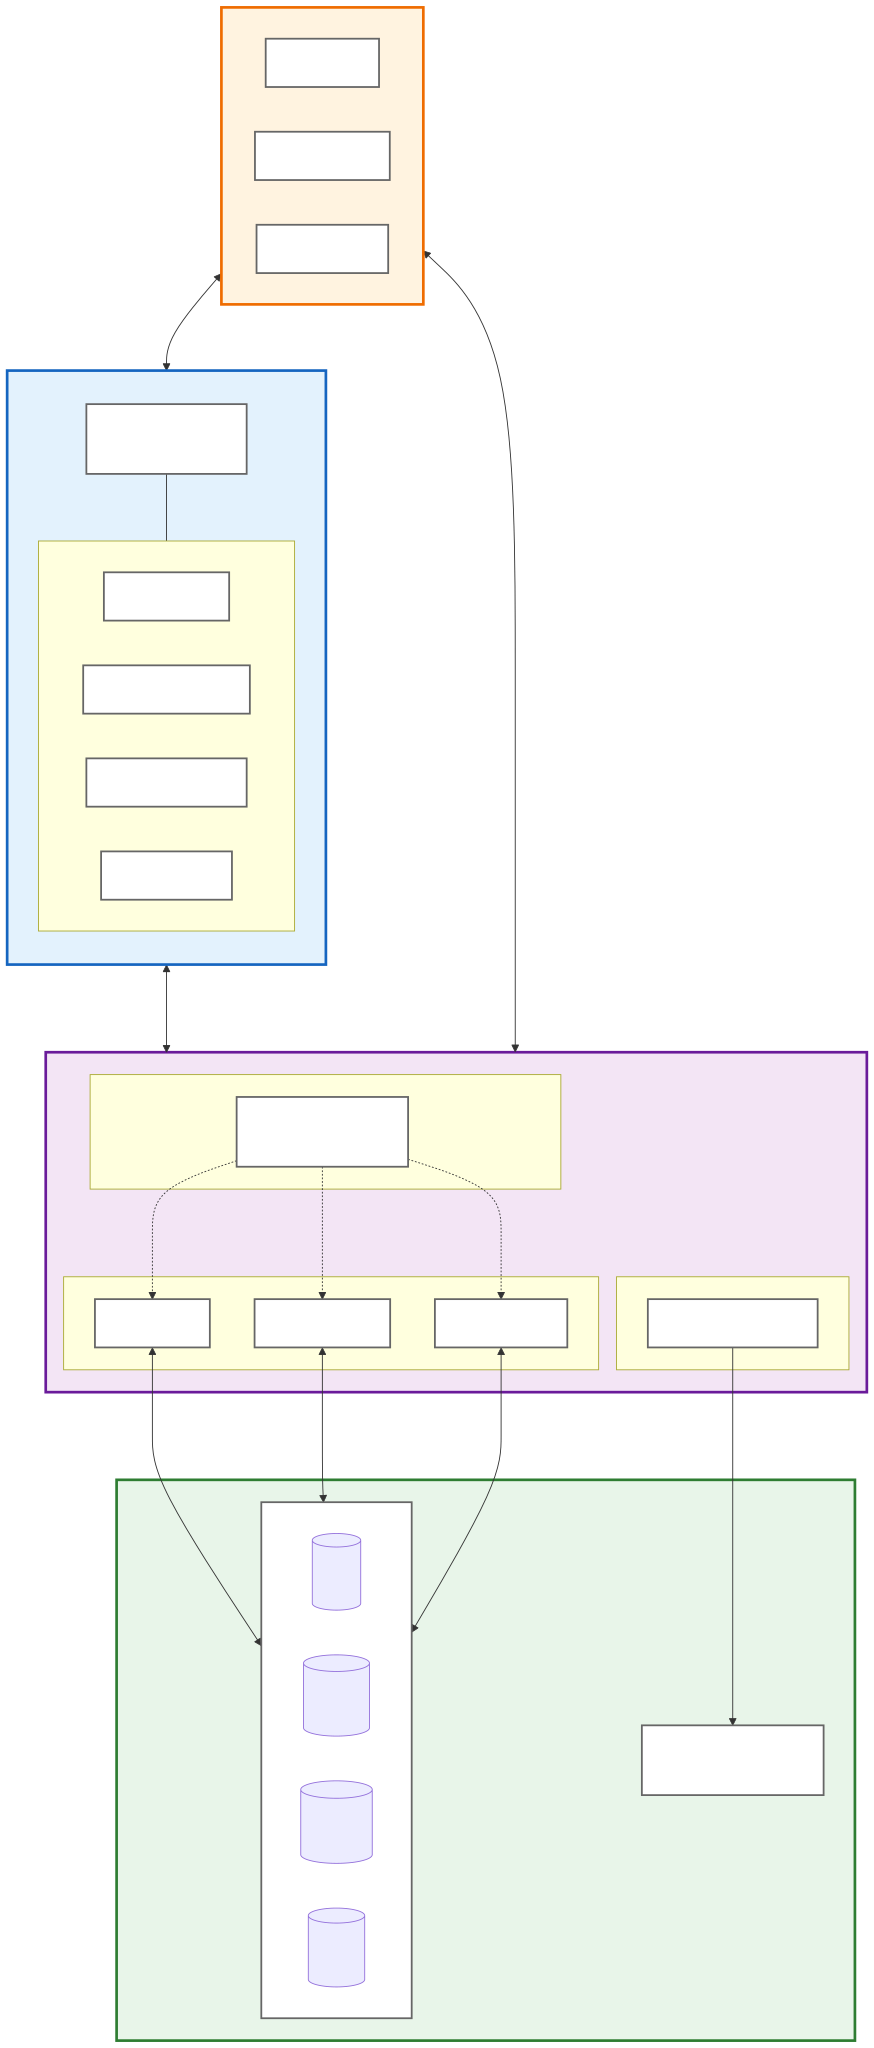
\includegraphics[width=0.8\textwidth]{images/architecture.jpeg}
    \caption{System Architecture of note0 Application}
    \label{fig:architecture}
\end{figure}

\subsection{Java Swing with FlatLaf}
The entire graphical user interface (GUI) for the note0 desktop application was built using \textbf{Java Swing} with \textbf{FlatLaf} for a modern dark theme. Swing is a mature and powerful GUI widget toolkit for Java that provides a rich set of components for creating interactive and platform-independent desktop applications. FlatLaf was chosen to provide a modern, professional appearance with a dark theme that enhances user experience. The framework's comprehensive library of components—such as \texttt{JFrame}, \texttt{JPanel}, \texttt{JTable}, and \texttt{JButton}—allowed for the creation of all necessary views, from the initial login and registration forms to the complex, data-driven dashboard. Swing's event-driven model was used to handle user interactions, such as button clicks and table selections, to trigger application logic.

\subsection{PostgreSQL (Cloud Hosted)}
For the data persistence layer, we selected \textbf{PostgreSQL}, a powerful, open-source object-relational database system renowned for its reliability, feature robustness, and data integrity. All application data—including user credentials, subject information, material metadata, and user ratings—is stored in a PostgreSQL database hosted on the Aiven cloud platform. This choice was deliberate; using a relational database ensures that the relationships between users, materials, and subjects are strictly maintained. The database schema is designed to be normalized to reduce redundancy. All interactions between the Java application and the database are handled via the standard PostgreSQL JDBC driver, which is specified as a dependency in our project's \texttt{pom.xml} file.

\subsection{Apache Maven}
\textbf{Apache Maven} is the build automation and project management tool used to structure and manage the entire lifecycle of the note0 project. Its primary role in this project is twofold. First, it handles \textbf{dependency management}. All external libraries required by the application, such as the PostgreSQL JDBC driver, the jBCrypt library for password hashing, and the Cloudinary SDK, are declared in the \texttt{pom.xml} file. Maven automatically downloads the correct versions of these libraries and makes them available to the project, which greatly simplifies the setup process. Second, Maven provides a standardized \textbf{build lifecycle}, automating tasks such as compiling the Java source code, managing resources, and executing the application. This ensures that the project is built in a consistent and repeatable manner across different development environments.

\section{Cloud Platform Integration}
To ensure scalability, reliability, and efficient data management, the note0 application leverages a strategic cloud-based infrastructure. Instead of relying on a single service, our architecture separates the hosting of the database from the management of digital content, using specialized platforms for each task. This approach ensures optimal performance and security for different types of data.

\subsection{Database Hosting - Aiven}
The core PostgreSQL database is hosted on \textbf{Aiven}, a managed cloud database service. Storing the database in the cloud rather than on a traditional server offers several significant advantages:
\begin{itemize}
    \item \textbf{High Availability and Reliability:} Aiven provides built-in redundancy and failover mechanisms, ensuring the database is almost always online and accessible.
    \item \textbf{Automated Backups:} The platform automatically handles regular backups of the database, which is critical for disaster recovery and preventing data loss.
    \item \textbf{Scalability:} If the application gains more users, the database resources (CPU, RAM, Storage) can be easily scaled up with minimal downtime.
    \item \textbf{Managed Security:} Aiven manages underlying security, patching, and network configuration, allowing our team to focus on application-level security.
\end{itemize}

\subsection{Digital Asset Management: Cloudinary}
For handling application materials such as user-uploaded files and attachments, we have integrated \textbf{Cloudinary}. Cloudinary is a specialized cloud platform for managing media assets. Using a dedicated service like Cloudinary instead of storing files directly on our server provides powerful benefits:
\begin{itemize}
    \item \textbf{Optimized Storage and Delivery:} Cloudinary stores assets on a highly efficient infrastructure and delivers them through a Content Delivery Network (CDN), meaning files load much faster for users anywhere in the world.
    \item \textbf{On-the-Fly Transformations:} It can automatically resize, crop, format, and apply effects to images via simple URL parameters. This removes the need for complex file processing logic in our Java backend.
    \item \textbf{Reduced Server Load:} By offloading the storage and serving of media files, Cloudinary significantly reduces the bandwidth and processing load on our primary application server, keeping it fast and responsive.
\end{itemize}

\section{Database Schema}
The database is designed to be simple yet effective, with four primary tables that support the application's functionality.

The main tables are:
\begin{itemize}
    \item \textbf{Users:} Stores user information, including a unique user ID, full name, email, hashed password, role (USER/ADMIN), college name, and semester information.
    \item \textbf{Subjects:} Stores academic subject information, including subject ID and name, managed through the admin panel.
    \item \textbf{Materials:} Stores information about each uploaded material, including material ID, title, file path (Cloudinary URL), average rating, upload timestamp, and foreign keys linking to the users and subjects tables.
    \item \textbf{Ratings:} A mapping table that stores each individual rating. It links a \texttt{user\_id} and a \texttt{material\_id} with a given score, creating a many-to-many relationship between users and materials.
\end{itemize}


%----------------------------------------------------------------------
%======================================================================
%   CHAPTER: Implementation and Testing
%   This chapter provides a detailed breakdown of the application's
%   core modules and the testing strategies employed.
%======================================================================

\chapter{Implementation and Testing}
The development of the note0 application was carried out in a modular fashion to ensure a clean separation of concerns and to facilitate maintainability. This chapter details the implementation of the key functional modules of the system. It also provides a comprehensive overview of the testing methodologies used to ensure the application's correctness, reliability, and performance.

%----------------------------------------------------------------------
\section{Module Implementation}
%----------------------------------------------------------------------
The application is logically divided into several modules, each responsible for a distinct set of functionalities. The implementation of these modules leverages the DAO (Data Access Object) pattern to isolate business logic from data persistence logic.

\subsection{User Authentication Module}
The User Authentication module is the security foundation of the note0 application, responsible for managing user identity and access control. It consists of two primary user-facing components—Registration and Login—supported by a robust backend Data Access Object.

\subsubsection{User Registration}
The registration process is handled by the \texttt{RegistrationPanel.java} class. This UI component provides fields for a user's full name, email, password, college name, and semester. Upon submission, the user's details, along with a securely hashed password using \textbf{jBCrypt}, are inserted into the \texttt{users} table in the PostgreSQL database.

\subsubsection{User Login}
The login process is managed by \texttt{LoginPanel.java}. When a user enters their credentials, the system queries the database for the user and uses \textbf{BCrypt.checkpw()} to securely compare the provided password against the stored hash. If valid, the \texttt{MainFrame} transitions the view to the main dashboard based on the user's role.

\subsection{Material Management and Sharing Module}
In this application, sharing is achieved by uploading a material to the central platform, making it accessible to all users. This module is primarily managed by \texttt{DashboardPanel.java} and \texttt{MaterialDAO.java}.

\subsubsection{Material Upload (Sharing)}
The process of sharing a new material involves the user providing metadata and a file, which is then uploaded to Cloudinary. The secure URL returned by Cloudinary is stored in the \texttt{materials} database table along with the metadata.

\subsubsection{Material Viewing, Rating, and Deletion}
Once uploaded, materials are managed through the dashboard. Users can view materials, which are dynamically loaded and filtered by the \texttt{MaterialDAO}. They can also rate materials using a 1-5 star rating system and delete materials (if they are the uploader or an admin), with all actions handled through database transactions to ensure data integrity.

\subsection{Admin Panel Module}
The admin panel is accessible only to users with the ADMIN role and provides functionality for managing subjects and overseeing the platform.

\subsubsection{Subject Management}
Administrators can add, edit, and delete subjects through the \texttt{AdminPanel.java} interface. This ensures that the subject dropdown in the material upload form is dynamically populated and managed centrally.

%----------------------------------------------------------------------
\section{Results and Screenshots}
%----------------------------------------------------------------------
The application successfully meets all the functional requirements outlined in the project objectives. The final system provides a stable and responsive desktop experience for sharing and managing academic materials. The user interface is intuitive, and the integration with cloud services for database and file storage ensures scalability and reliability.

\subsection{Application Screenshots}
The following figures provide a visual overview of the application's main interfaces.
\begin{figure}[h!]
    \centering
    \includegraphics[width=0.6\textwidth]{new_images_note/login_page.png}
    \caption{Login and Registration Interface}
    \label{fig:login_page}
\end{figure}

\begin{figure}[h!]
    \centering
    \includegraphics[width=0.6\textwidth]{new_images_note/home_page.png}
    \caption{The Home Page of Note0 application}
    \label{fig:home_page}
\end{figure}

\begin{figure}[h!]
    \centering
    \includegraphics[width=0.6\textwidth]{new_images_note/browse_page.png}
    \caption{The Browse Page: Main Dashboard for Materials}
    \label{fig:browse_page}
\end{figure}

\begin{figure}[h!]
    \centering
    \includegraphics[width=0.6\textwidth]{new_images_note/browse_upload.png}
    \caption{The Browse Page: To Upload Materials}
    \label{fig:browse_upload}
\end{figure}

\begin{figure}[h!]
    \centering
    \includegraphics[width=0.6\textwidth]{new_images_note/profile_page.png}
    \caption{The User Profile View (Welcome Area)}
    \label{fig:profile_page}
\end{figure}

\begin{figure}[h!]
    \centering
    \includegraphics[width=0.6\textwidth]{new_images_note/admin_page.png}
    \caption{The Admin Page for Subject Management}
    \label{fig:admin_page}
\end{figure}

\subsection{Testing Strategy}
A multi-layered testing strategy was employed to ensure the quality and correctness of the application. This strategy included unit testing, integration testing, and user acceptance testing.

\subsubsection{Unit Testing}
Unit tests were designed to verify the functionality of individual methods in isolation, particularly within the Data Access Object (DAO) classes and utility methods.

\subsubsection{Integration Testing}
Integration testing focused on verifying the interaction between different layers of the application, from a UI event (like a button click) to the database response and cloud service integration.

\subsubsection{User Acceptance Testing (UAT)}
UAT was performed manually to ensure the application meets the end-user's requirements and is free of major usability issues.

\begin{table}[h!]
    \centering
    \caption{Test Cases for User Authentication}
    \label{tab:auth_tests}
    \begin{tabular}{|p{1cm}|p{4.5cm}|p{4.5cm}|p{2cm}|}
        \hline
        \textbf{ID} & \textbf{Test Case Description} & \textbf{Expected Result} & \textbf{Status} \\
        \hline
        TC-01 & User enters valid email and password. & User is successfully logged in and the dashboard is displayed. & Pass \\
        \hline
        TC-02 & User enters a valid email but an incorrect password. & An "Invalid email or password" error message is shown. & Pass \\
        \hline
        TC-03 & Admin user logs in with valid credentials. & Admin user is logged in and admin panel is accessible. & Pass \\
        \hline
    \end{tabular}
\end{table}

\begin{table}[h!]
    \centering
    \caption{Test Cases for Material Management}
    \label{tab:material_tests}
    \begin{tabular}{|p{1cm}|p{4.5cm}|p{4.5cm}|p{2cm}|}
        \hline
        \textbf{ID} & \textbf{Test Case Description} & \textbf{Expected Result} & \textbf{Status} \\
        \hline
        TC-04 & User successfully uploads a new PDF file. & The file appears in the dashboard table with Cloudinary URL. & Pass \\
        \hline
        TC-05 & Admin user logs in and deletes a subject. & The subject is removed and no longer appears in the dashboard filters. & Pass \\
        \hline
        TC-06 & User rates a material with 4 stars. & The rating is saved and average rating is updated. & Pass \\
        \hline
    \end{tabular}
\end{table}

\chapter{Conclusion and Future Scope}
%----------------------------------------------------------------------

\section{Conclusion}
We successfully achieved our primary goal of developing \textbf{note0}, a collaborative material-sharing platform that directly addresses the challenges of resource scarcity and fragmented information in academic environments.

The project successfully integrated Java Swing with FlatLaf, PostgreSQL database hosted on Aiven, and Cloudinary for file storage to create a robust and scalable solution. Maven was instrumental in managing our project's dependencies and build cycle, ensuring a smooth and standardized development process. The implementation of role-based access control, secure authentication with jBCrypt, and cloud integration demonstrates the application's enterprise-ready architecture.

Key achievements include:
\begin{itemize}
    \item Successful implementation of a layered architecture with clear separation of concerns
    \item Secure user authentication with password hashing
    \item Role-based access control distinguishing between users and administrators
    \item Cloud integration for both database hosting and file storage
    \item Modern, responsive user interface with dark theme
    \item Comprehensive material management with rating system
\end{itemize}

In conclusion, \textbf{note0} is not just a functional application; it is a proof-of-concept for how technology can bridge gaps in educational resources and foster a more collaborative learning environment.

\section{Future Scope}
The note0 application currently serves as a robust proof-of-concept and a functional platform for sharing academic materials. The existing architecture provides a solid foundation upon which a wide range of advanced features can be built. The following enhancements are identified as a roadmap for the future development of the project.

\subsection{Cross-Platform Accessibility}
The most significant enhancement would be to evolve note0 from a desktop-only application into a full-fledged cross-platform service.
\begin{itemize}
    \item \textbf{Web Application:} Developing a web-based client using a modern framework (like React or Angular) would make the platform accessible from any device with a web browser, removing the need for a local installation.
    \item \textbf{Mobile Applications:} Creating native mobile applications for Android and iOS would provide users with on-the-go access to their materials, a critical feature for students.
\end{itemize}

\subsection{Advanced Collaboration Features}
To transform the application from a simple sharing platform into a truly collaborative tool, the following features could be implemented:
\begin{itemize}
    \item \textbf{Real-Time Editing:} By integrating technologies like WebSockets, the platform could be enhanced to support simultaneous editing of a single document by multiple users, similar to the functionality of Google Docs.
    \item \textbf{Commenting and Annotation:} Allowing users to leave comments and annotations on specific parts of a document would greatly improve collaborative feedback and discussion.
    \item \textbf{Version History:} Implementing a system to track changes and allow users to revert to previous versions of a material would prevent accidental data loss and provide a clear history of contributions.
\end{itemize}

\subsection{Enhanced User Experience and Organization}
Improving the user's ability to manage and find their content is crucial for long-term usability.
\begin{itemize}
    \item \textbf{Folder and Tagging System:} Instead of a single list of materials, users could organize their notes into folders and sub-folders. A tagging system would also allow for more flexible, non-hierarchical organization.
    \item \textbf{Advanced Search:} The current search functionality could be expanded to include full-text search within documents, as well as filtering by date, uploader, rating, and other metadata.
    \item \textbf{Notifications:} A notification system could alert users when a new material is uploaded in a subject they follow, or when another user comments on or rates their contribution.
\end{itemize}

\subsection{Offline Functionality}
To improve accessibility, offline support could be implemented. This would involve creating a local cache or database (e.g., using SQLite) on the user's machine. Users could then view, create, and edit their materials without an active internet connection. All changes would be synchronized with the central cloud database automatically once the user goes online.

%======================================================================
%   ix. APPENDICES
%======================================================================
\appendix
\chapter{Sample Code Snippet: Database Connectivity}

A critical component of the backend is its ability to communicate with the cloud-hosted PostgreSQL database. This is handled by the \texttt{DatabaseManager.java} class, which uses the Java Database Connectivity (JDBC) API. The following code snippet shows the implementation for establishing this connection.

\begin{verbatim}
package com.note0.simple;

import java.sql.Connection;
import java.sql.DriverManager;
import java.sql.SQLException;

public class DatabaseManager {

    // --- IMPORTANT: REPLACE THESE WITH YOUR AIVEN CREDENTIALS ---
    private static final String DB_URL = "jdbc:postgresql://pg-1f5358eb-note0.k.aivencloud.com:17737/defaultdb?sslmode=require";
    private static final String USER = "avnadmin";
    private static final String PASSWORD = "AVNS_zjes6XbHRJo9YtEPMuI";
    // -----------------------------------------------------------

    public static Connection getConnection() throws SQLException {
        return DriverManager.getConnection(DB_URL, USER, PASSWORD);
    }
}
\end{verbatim}

\chapter{Detailed Code Explanation: DashboardPanel.java}
\addcontentsline{toc}{chapter}{Appendix B: Detailed Code Explanation}

The \texttt{DashboardPanel.java} class is the functional core of the note0 application's user interface. After a user successfully authenticates, this panel is displayed and serves as the primary workspace for all material management and interaction. It is an excellent example of the Model-View-Controller (MVC) principle, where the Swing components act as the 'View', and this class acts as the 'Controller', mediating between the UI and the 'Model' (the DAO classes).

The responsibilities of the \texttt{DashboardPanel} can be broken down into three main areas: UI construction, data management, and event handling.

\section{UI Construction and Layout}
The visual structure of the dashboard is built using a combination of Swing layout managers to create a responsive and organized interface. The main panel uses a \texttt{BorderLayout} to divide the screen into distinct regions.

\begin{itemize}
    \item \textbf{NORTH Region:} The top panel, created by the \texttt{createTopPanel()} method, contains a welcome message, a logout button, filters for searching, and, conditionally, an "Admin Panel" button that only appears if the logged-in user has the `ADMIN` role.
    \item \textbf{CENTER Region:} This is the largest area, containing the \texttt{JTable} that displays the list of materials. It is wrapped in a \texttt{JScrollPane} to allow for scrolling when the content exceeds the viewable area.
    \item \textbf{SOUTH Region:} The bottom panel, created by \texttt{createBottomPanel()}, contains the form for uploading new materials, including fields for the title, a subject selector, and buttons for choosing a file and initiating the upload.
\end{itemize}

\section{Data Management and Display}
A key function of the dashboard is to fetch data from the database and present it to the user. This is primarily handled by the \texttt{loadMaterialsIntoTable()} method.

\begin{figure}[h!]
\begin{verbatim}
private void loadMaterialsIntoTable() {
    tableModel.setRowCount(0); // Clear the table first
    try {
        String titleFilter = searchField.getText().trim();
        String branchFilter = ...;
        int semesterFilter = ...;
        String subjectFilter = ...;

        List<Material> materials = materialDAO.getMaterials(
            titleFilter, branchFilter, semesterFilter, subjectFilter);
            
        for (Material material : materials) {
            tableModel.addRow(new Object[]{
                material.getId(), material.getTitle(), 
                material.getSubjectName(), material.getUploaderName(), 
                String.format("%.2f", material.getAverageRating())
            });
        }
    } catch (SQLException e) {
        JOptionPane.showMessageDialog(this, "Could not load materials: " 
            + e.getMessage(), "DB Error", JOptionPane.ERROR_MESSAGE);
    }
}
\end{verbatim}
\caption{Method for loading and filtering materials from the database.}
\label{fig:load_materials}
\end{figure}

As shown in Figure \ref{fig:load_materials}, this method demonstrates a complete data retrieval workflow:
\begin{enumerate}
    \item It begins by clearing any existing data from the table model to ensure a fresh display.
    \item It collects the current values from all filter components (search field, subject dropdown, etc.).
    \item It calls the \texttt{materialDAO.getMaterials(...)} method, passing the filter criteria. The DAO is responsible for dynamically building the appropriate SQL query to fetch the correct subset of data from the PostgreSQL database.
    \item Finally, it iterates through the returned list of \texttt{Material} objects and populates the \texttt{JTable} row by row.
\end{enumerate}

\section{Event Handling: Material Upload}
The process of uploading a new material is an excellent example of how the panel handles a complex user action involving file I/O, cloud services, and database interaction. This logic resides in the \texttt{handleUpload()} method.

\begin{figure}[h!]
\begin{verbatim}
private void handleUpload() {
    if (titleField.getText().isBlank() || selectedFile == null || ...) {
        // Input validation...
        return;
    }
    try {
        // 1. Generate a unique ID for the cloud asset
        String publicId = UUID.randomUUID().toString();

        // 2. Call the Cloudinary service to upload the file
        String url = cloudinaryService.uploadFile(selectedFile, 
            "note0/materials", publicId);
        
        // 3. Get the subject ID from the UI
        String selectedSubjectName = (String) uploadSubjectComboBox.getSelectedItem();
        long subjectId = subjectNameToIdMap.get(selectedSubjectName);
        
        // 4. Call the DAO to save metadata to the database
        materialDAO.addMaterial(titleField.getText(), url, subjectId, 
            loggedInUser.getId());
        
        JOptionPane.showMessageDialog(this, "Upload successful!", "Success", ...);
        loadMaterialsIntoTable(); // Refresh the table
    } catch (Exception ex) {
        // Error handling...
    }
}
\end{verbatim}
\caption{The event handler for uploading a new material.}
\label{fig:handle_upload}
\end{figure}

The workflow, illustrated in Figure \ref{fig:handle_upload}, is as follows:
\begin{enumerate}
    \item The method first performs input validation to ensure all required fields are filled and a file has been selected.
    \item A unique identifier is generated for the file to prevent naming conflicts in the cloud storage.
    \item The \texttt{cloudinaryService} is called to handle the actual file upload. This service abstracts away the complexity of interacting with the Cloudinary API.
    \item Upon a successful upload, Cloudinary returns a secure URL for the hosted file. This URL, along with other metadata like the title and subject ID, is then passed to the \texttt{materialDAO} to be saved in the database.
    \item Finally, a success message is shown to the user, and the main table is refreshed to include the newly added material.
\end{enumerate}

%======================================================================
%   x. REFERENCES
%======================================================================
\begin{thebibliography}{9}
\addcontentsline{toc}{chapter}{References}

\bibitem{java_docs}
Oracle Corporation, "Java SE 17 Documentation", 2023. [Online]. Available: https://docs.oracle.com/en/java/javase/17/

\bibitem{swing_tutorial}
Kathy Sierra and Bert Bates, "Head First Java", 2nd Edition, O'Reilly Media, 2005.

\bibitem{maven_guide}
Apache Maven Project, "Maven: The Definitive Guide", Sonatype, 2008. [Online]. Available: https://maven.apache.org/guides/

\bibitem{postgresql_docs}
PostgreSQL Documentation Team, "PostgreSQL 15 Documentation", PostgreSQL Global Development Group, 2024.

\bibitem{flatlaf_docs}
FormDev Software, "FlatLaf - Flat Look and Feel", 2023. [Online]. Available: https://github.com/JFormDesigner/FlatLaf

\bibitem{cloudinary_docs}
Cloudinary Ltd., "Cloudinary Documentation", 2024. [Online]. Available: https://cloudinary.com/documentation

\bibitem{aiven_docs}
Aiven Ltd., "Aiven PostgreSQL Documentation", 2024. [Online]. Available: https://docs.aiven.io/docs/products/postgresql

\bibitem{bcrypt_docs}
Mindrot, "jBCrypt - A Java implementation of OpenBSD's Blowfish password hashing code", 2024. [Online]. Available: https://github.com/jeremyh/jBCrypt

\end{thebibliography}

%======================================================================
%   3. DOCUMENT END
%======================================================================
\end{document}
